Our beliefs about political issues are not entirely independent of each other; they are embedded and structured within personal belief systems. For example, Alice's concern about climate change may constrain her position on economic growth; Bob's similar concern about climate change might, however, not conflict with his belief that technological advances will foster economic growth. We can model such individual-level systems as networks of beliefs: nodes represent an individual's beliefs on specific issues and edges represent (positive or negative) relations, influences, or constraints between these items. Recent research has focussed predominantly on exploring how individuals change (or resist changing) their beliefs, given that beliefs are structured in a network \cite{baumannEmergencePolarizedIdeological2021, brandtEvaluatingBeliefSystem2021, friedkinNetworkScienceBelief2016, dalegeNetworksBeliefsIntegrative2025}. These studies typically assumed that the individuals' belief networks are prescribed (for example, based on logical relation), static, and homogeneous. Much less work has focused on how such belief network structures adapt and evolve over time, how they potentially diverge across individuals, and what the consequences of such dynamic heterogeneity is. This is our goal in this modelling study.

Our computational model extends the Networks of Beliefs (NB) theory, proposed in \citet{dalegeNetworksBeliefsIntegrative2025}. The original theory described how individuals update their beliefs when they experience dissonance (either with other personal beliefs, with social beliefs or between social beliefs and external signals) in a statistical physics framework. In our extension, individuals update not only their beliefs but also their personal belief network structure, i.e.~they change the weights of edges that connect personal beliefs. Adaptation of edges occurs through two processes. The first process represents social conformity---when others see a strong (or no) relation between two beliefs, it is difficult to ignore (or maintain) this relation individually. The second process represents internal learning---when two beliefs of an individual consistently change in the same direction (i.e.~when they both become more extreme in the same direction), the individual will perceive a stronger relation between these beliefs. 

\begin{figure}[h]
    \centering
    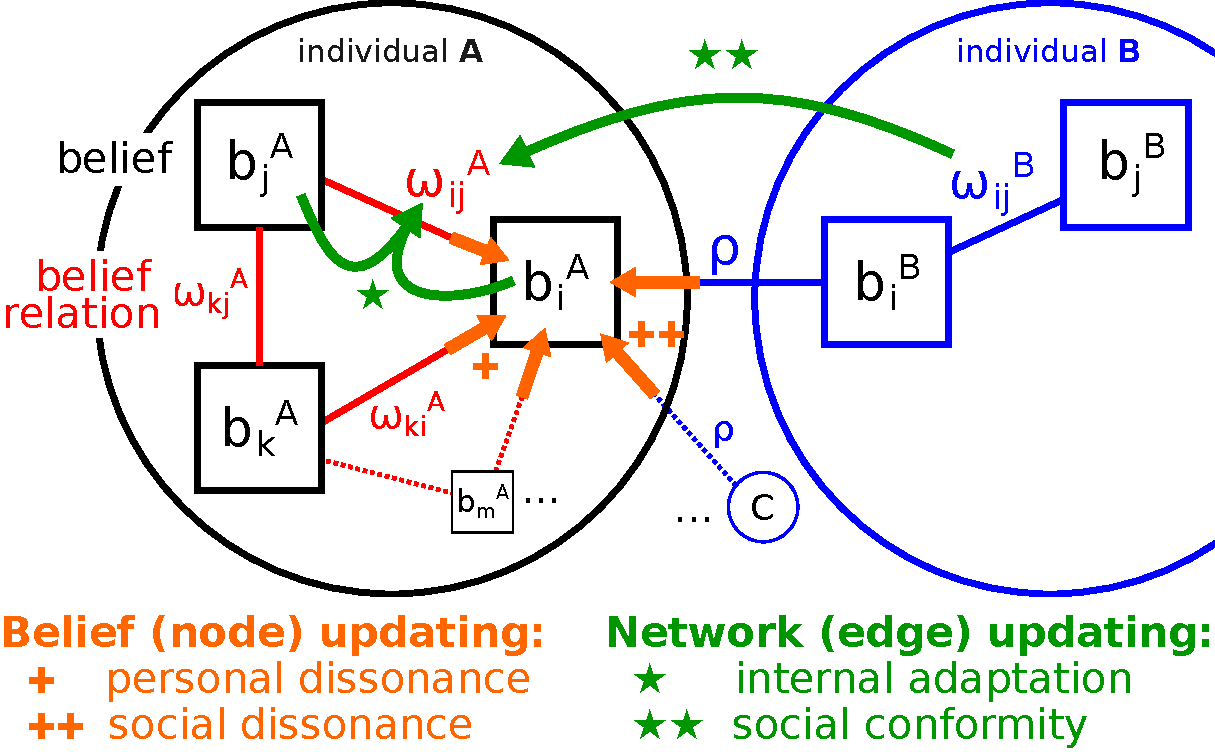
\includegraphics[width=0.5\linewidth]{full_sketch_+beliefUpdate+edgeUpdate.pdf}
    \caption{Sketch of the adaptive belief network model. Orange arrows indicate influences on the agent $A$'s (here, focal) belief $b_i$, in line with the proposed model by \citet{dalegeNetworksBeliefsIntegrative2025}; green arrows indicate influences on the edge $\omega_{ij}$.}
    \label{fig:sketch}
\end{figure}

We explore how changes in belief networks can lead to heterogeneity among individuals, and how this affects polarisation and consensus patterns: What are the conditions under which plasticity of belief networks leads to heterogeneity in peoples' belief networks? Does the emergence of heterogeneity in belief networks depend on or contribute to ideological polarisation? We also explore consequences of evolved belief networks heterogeneity, in particular its effects on individuals' responses to external pressures: Can heterogeneity in belief networks (not in beliefs) explain why some people respond quite drastically to belief interventions or disruptive (political) events, while others' beliefs (and belief systems) remain robust? 

\subsection*{Model}

In the following, we describe the base model as proposed by \citet{dalegeNetworksBeliefsIntegrative2025} and our extension to adaptive belief networks in this study in more detail. Each agent has ten beliefs, $b\in\{-1, -0.67, -0.33, 0, 0.33, 0.67, 1\}$, indicating agreement or disagreement about ten political items. One of these belief items is the \textit{focal belief}. You may think of this as nine hidden or abstract beliefs, such as beliefs about the extent of climate change, the causes of it, and responsibility for the development, and one specific overt focal belief, for example, about the best value for a carbon tax---a belief that many people debate and observe in their peers. The belief network describes how the agent thinks these beliefs should be aligned or disaligned (details later). We intialise the agents' belief networks as fully connected, i.e.\ each belief $i$ of agent $A$ is connected to all its other personal beliefs $j$ with edge weights $\omega_{ij} = \omega_0$. While non-focal beliefs are private, the focal belief is shared with and influenced by the agent's neighbours in a social network. In all simulations, we use a fixed social network generated from a Stochastic Block Model with two equally sized groups, 'G1' and 'G2' (link probability $40\,\%$ between agents of the same group and $1\,\%$ between agents of different groups; otherwise agents from different groups are identical). The focal belief of an agent is then not only connected to non-focal personal beliefs, but also to the focal beliefs of social network neighbours of the agents with edge weight $\rho$ (see sketch in Figure~\ref{fig:sketch}). A belief network relation can increase or decrease the agent's feeling of dissonance depending on if the connected beliefs are misaligned or aligned. Using the analogy of energy in spin systems, and in line with \citeauthor{dalegeNetworksBeliefsIntegrative2025}, we determine the dissonance between beliefs $i$ and $j$ as $H_{pers, ij} = \omega_{ij} \cdot b_i \cdot b_j$ or, in sum, 
\begin{equation}
H_{pers} = \sum_{ij} \omega_{ij} \cdot b_i \cdot b_j
\end{equation}
for all edges $(i,j)$ between personal beliefs and 
\begin{equation}
H_{soc} = \sum_{nb} \rho \cdot b_{\rm focal} \cdot b^{\rm nb}_{\rm focal}
\end{equation}
for all edges connecting the focal belief of the agent to focal beliefs of other agents. In each time step of a simulation, agents update all beliefs (in random order) based on the total dissonance $H = H_{\rm pers} + H_{\rm soc}$. The agent considers all possible beliefs $b'$ on a given item $i$ and changes its belief to $b'$ with probability $p(b \rightarrow b') = 1 / \left(1+\exp(H(b') - H(b))\right)$, i.e.\ agents tend to favour beliefs that minimise dissonance. This model so far follows closely the model proposed in \citet{dalegeNetworksBeliefsIntegrative2025}. 

In the following, we describe how agents adapt the edge weights of their belief network (see also sketch in Figure~\ref{fig:sketch}) via internal and social processes. We formalise the internal process as Hebbian learning: agents learn to strengthen/weaken those relations that connect beliefs that consistently/inconsistently change in the same direction. We formalise social conformity as a convergence of an edge in the agent's personal belief network towards the corresponding edge of the agent's peers. In each time step of the simulation, an agent $A$ updates all belief network edge weights $\omega_{ij}^A$ (in random order) as 
\begin{equation}
\omega_{ij}^A = \omega_{ij}^A + \mu \cdot (\omega_{ij}^B - \omega_{ij}^A) + \epsilon \cdot \partial b_{i} \cdot \partial b_{j} \ ,
\end{equation}
where $B$ is a randomly drawn neighbouring agent of $A$, $\mu$ is a parameter describing the strength of social conformity, $\epsilon$ is a parameter describing the strength of internal learning and $\partial b_i$ describes the direction and degree of change of the individuals' belief $i$ over the previous $3$ time steps. For example, if $b_i$ has decreased from $1$ to $0$ to $-0.33$ to $-1$ in the past three time steps, then $\partial b_i = \frac{-1-0.33-0.67}{3} = -0.67$. IN this case, internal learning would increase the edge weight $\omega_{ij}^A$ in agent $A$'s belief network if its belief $b_j$ would have decreased as well, $\partial b_j<0$, and learning would decrease this edge weight if $\partial b_j>0$. 


\begin{figure}[t]
    \centering
    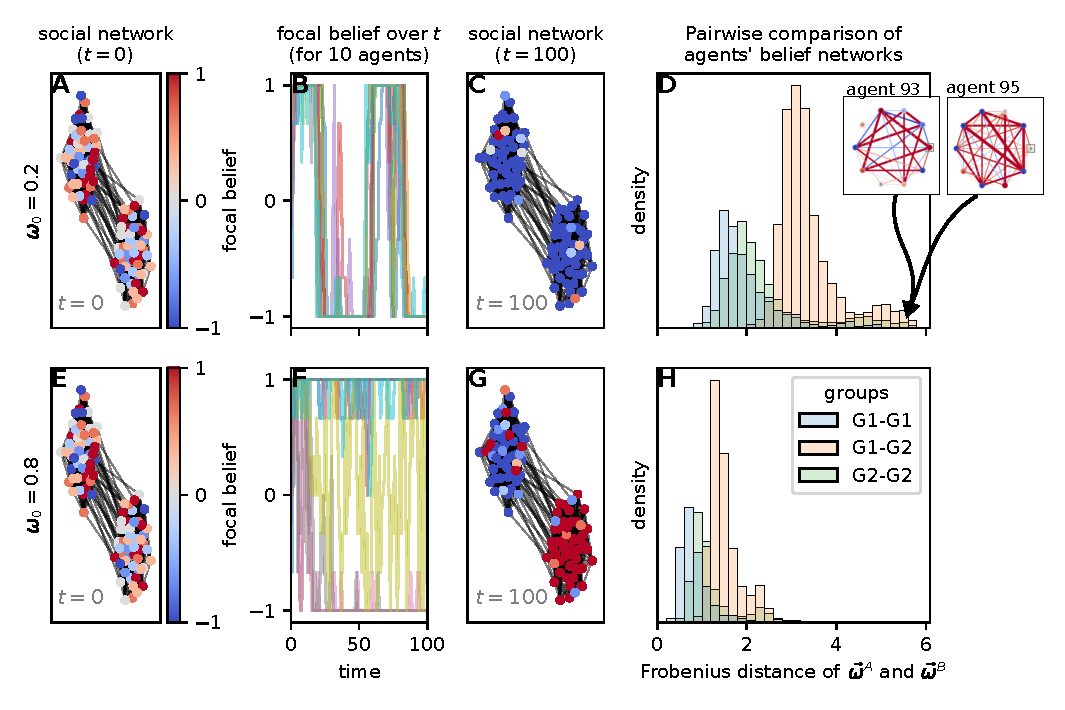
\includegraphics[width=0.8\linewidth]{figures/dynamics_adaptiveNB+inset.pdf}
    \caption{Focal belief and belief network dynamics for example simulations with adaptive networks ($\epsilon=0.3$ and $\mu=0.5$) and with low initial weights ($\omega_0=0.2$, top row) or high initial weights ($\omega_0 = 0.8$, bottom row). \textbf{A} and \textbf{E)} initial focal beliefs of agents in the social network, which is comprised of two social clusters 'G1' and 'G2'. Each dot represents one agent; links represent the social connections. \textbf{B} and \textbf{F)} dynamics of the focal beliefs for ten exemplary agents from both groups. \textbf{C} and \textbf{G)} focal beliefs after $t=100$ time steps. \textbf{D} and \textbf{H)} differences in the edge weights of the agents' belief networks at $t=100$. The bars show the frequency of the Frobenius distances obtained by comparing two agents' belief networks either within agents of the same group (G1-G1 and G2-G2) or between agents of different groups (G1-G2). High Frobenius distance indicates that the agents have very distinct belief network structures. The inset panels illustrate examples of two very distinct belief networks (colour and width of the edges represents the weights in the belief network).}
    \label{fig:res1}
\end{figure}

\section*{Results} 

\subsection*{Adaptive vs.~Fixed Belief Networks}

Figure \ref{fig:res1} shows the results of a single simulation of our model extension with low and high initial belief network edges ($\omega_0=0.2$ or $0.8$): from the initial focal beliefs of the agents in the social network (left column panels), exemplary dynamics of some of the agents' focal opinions over time (2nd column panels), to the focal beliefs of the agents after $t=100$ time steps (3rd column panels). The simulation with higher initial edge weights, $\omega_0=0.8$, produces stronger group polarisation in this particular scenario; however, this outcome varies a lot over different random simulations. The important aspect is that even though the focal beliefs are aligned across the agents in the simulation with $\omega_0=0.2$ (panel C), the belief networks of the agents differ a lot (right column panels), especially between agents of different social groups. We show, as an example, the evolved belief networks of two agents with very different belief network structures in this simulation (grey inset panels). Depending on the initial conditions, in some simulations (not shown), one of the two group develops a shared network with all agents having equivalent belief networks (and zero Frobenius distance), while the other group evaluate very different edges in their respective belief networks.  

Figure \ref{fig:outcomes} shows macro-level outcome patterns for the focal beliefs (top row) and the belief network edges (bottom row). The indicators for the focal beliefs (standard deviation, average extremeness, and modularity) are relatively consistent with fixed (light colors) as well as with adaptive networks (dark colours) for both scenarios, initialising belief networks with low and with high edge weights (blue, green). However, the belief networks (by design) remain static and homogeneous in the original model (with $\mu=\epsilon=0$), while they become heterogeneous in our adaptive version of the belief networks model (here with $\epsilon=0.3$ and $\mu=0.5$). This heterogeneity manifests in the macro-level indicators for the edges of the belief networks (bottom row), such as increased standard deviation of edges across participants, average extremeness of the edges (starting from the initial $\omega_{0} = 0.2$ or $0.8$), and increased differences in belief network, especially across groups. In this case, although the focal beliefs might be shared, individuals hold these beliefs with a very different belief network `in the background'. Also notably, belief network differences become especially pronounced when the initial edge weights are small. In sum, belief dynamics and belief network divergence may not be fully coupled. 


\begin{figure}[t]
    \centering
    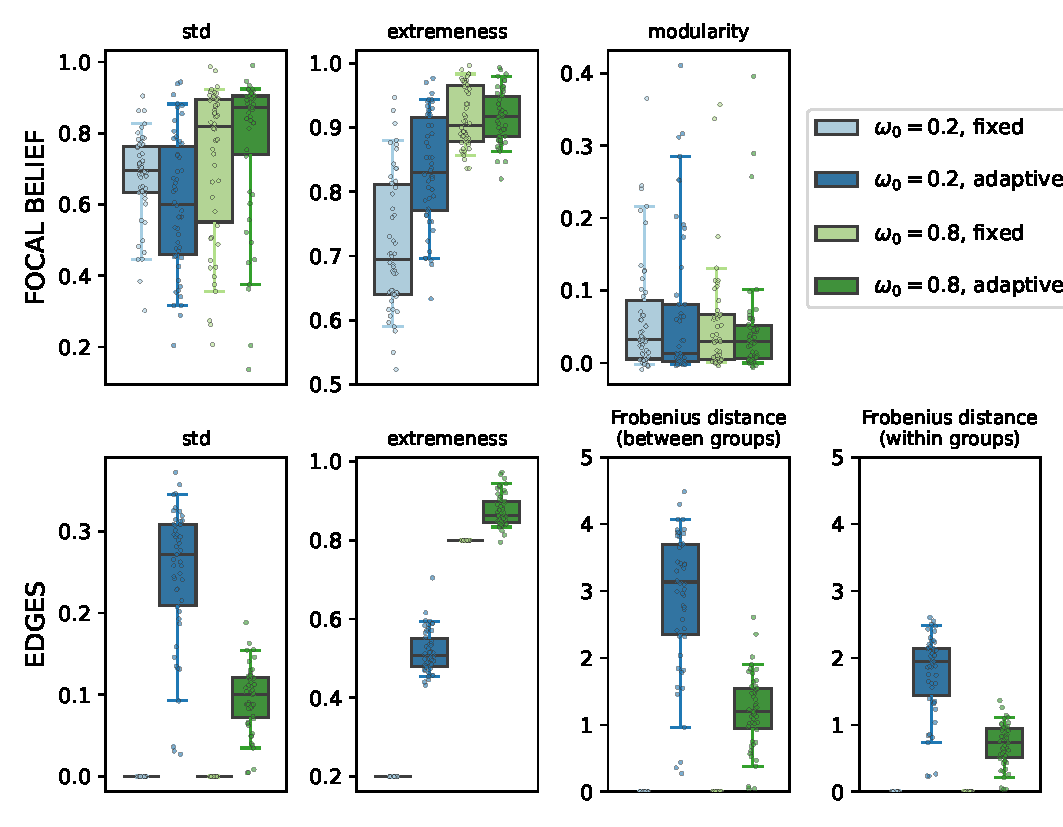
\includegraphics[width=0.8\linewidth]{figures/outcomes.pdf}
    \caption{Macro-level outcome measures for 50 simulations with fixed ($\mu=0$, $\epsilon=0$; light colours) and with adaptive belief networks ($\mu=0.5$, $\epsilon=0.3$; dark colours). As before, we test two scenarios: low initial weights, $\omega_0=0.2$ (blue), and high initial weights, $\omega_0=0.8$ (green). For the focal beliefs, the outcome measures include: \textbf{A)} standard deviation across the agents' focal beliefs, \textbf{B)} average extremeness of their focal beliefs, and \textbf{C)} modularity of the focal beliefs in the social network. For belief network edges, the measures include: \textbf{D)} average standard deviation across agents, \textbf{D)} average extremeness of the edge weights in the belief networks, \textbf{E} and \textbf{F)} average frobenius distances of belief networks between agents in different (orange) or the same social groups (green and blue).}
    \label{fig:outcomes}
\end{figure}

\subsection*{Outlook to Interventions}

We are currently exploring how interventions affect the dynamics of beliefs and belief systems, given that agents have developed quite heterogeneous belief network structures. In the next months, we will systematically identify and illustrate conditions under which external pressures (either on the focal node or on non-focal nodes, as well as on edges in the belief networks) can lead to different agent responses in the two social clusters. For example, we expect that a sudden pressure to change a non-focal belief (e.g.~after learning about a scandal involving a certain politician, a natural crisis, or increased media attention to a specific issue) may cause dissonance and thus belief/belief network change for some individuals, but not for all. This could pave a way to better understand the co-existence of robustness and lack thereof after disruptive event or intervention even among individuals who ostensibly hold similar focal beliefs and express similar opinions.   

\section*{Concluding Remarks}

In this study, we shifted the focus of a belief dynamics model to an often overlooked aspect of it: people tend to organise multiple beliefs within belief networks that can reassure or cause dissonance, but rather than just adopting beliefs to reduce dissonances in isolation, the way beliefs are organised can also change \cite{fishmanChangeWeCan2022} and differ greatly between people \cite{baldassarriNeitherIdeologuesAgnostics2014, ludersAttitudeNetworksIntergroup2024, goldbergSocialContagionAssociative2018}. We show how plasticity of belief networks can induce heterogeneity across a population of agents even within groups of agents with similar opinions, thus, likely leading to a situation where interventions on these agents may be effetive on some agents but not on others. Even though observable belief patterns may not be affected by the belief network adaptation, such dynamics can lead to `hidden' psychological dynamics `in the background' that may eventually become critical. We hope that this modelling study inspires researchers to look beyond (overt) belief dynamics in isolation and to allow for co-evolution of beliefs and belief networks.   

